\documentclass[aps,prd,twocolumn,superscriptaddress,nofootinbib]{revtex4-2}

\usepackage{amsmath,amssymb}
\usepackage{graphicx}
\usepackage{xcolor}
\usepackage{hyperref}
\hypersetup{colorlinks=true,linkcolor=blue!60!black,citecolor=blue!60!black,urlcolor=blue!60!black}

\newcommand{\todo}[1]{\textcolor{red!70!black}{[TODO: #1]}}
\newcommand{\qqbar}{q\bar{q}}
\newcommand{\Teff}{T_{\mathrm{eff}}}
\newcommand{\Tchem}{T_{\mathrm{chem}}}
\newcommand{\Tcc}{T_{cc}^{+}}
\newcommand{\chic}{\chi_{c1}(3872)}
\newcommand{\fm}{\,\mathrm{fm}}
\newcommand{\GeV}{\,\mathrm{GeV}}
\newcommand{\MeV}{\,\mathrm{MeV}}

\begin{document}

\title{How Often Do Multiquark Hadrons Form?\\
Species Ratios from a Dynamical Quark Gas and a Renormalizable
Framework for Quantum Simulations}

\author{Henry Lamm}
\email{hlamm@fnal.gov}
\affiliation{Fermi National Accelerator Laboratory, Batavia, Illinois, 60510, USA}

\date{\today}

\begin{abstract}
Lebed's nearest-neighbor estimate [Phys.\ Rev.\ D \textbf{94}, 034039 (2016)]
suggested that diquark formation in a quark--antiquark gas is common, with
probabilities of tens of percent.  We extend this static counting in two
directions.  First, we perform dynamical classical simulations of an
expanding quark--antiquark plasma with discrete color charges,
Casimir-weighted screened interactions, Poisson-hazard annihilation into
gluonic and electromagnetic channels with tunable timescales, and thermal
flavors, measuring the meson\,:\,baryon\,:\,tetraquark\,:\,pentaquark ratios
that emerge at freeze-out together with the fraction of baryons that form
through a diquark intermediate.  Second, we formulate a rigorous
measurement framework through which the same species ratios become
renormalization-group-safe observables of a real-time $3{+}1$D lattice-QCD
quantum simulation of a fireball quench: integer-quantized conserved
charges and spectral data read out on spatially isolated color-singlet
clusters, organized in a four-tier hierarchy that separates
scheme-independent state counting from deliberately scheme-labeled
structure diagnostics.  In production ensembles ($N=3000$) the yield
ladder is strikingly non-geometric --- meson$\to$baryon costs
$\sim65\times$ but baryon$\to$tetraquark only $\sim5\times$ --- the
strong-coupling corner produces manifestly flavor-exotic,
strangeness-rich tetraquarks at $0.29\pm0.11$ per event (with
$cc\bar q\bar q$ production bounded), and the fraction of baryons that
form through
a persistent diquark intermediate is $0.91$--$0.95\pm0.02$ across all
expansion rates and couplings scanned: dynamics \emph{amplifies}
Lebed's static estimate by more than a factor of three.
\end{abstract}

\maketitle

\section{Introduction}
\label{sec:intro}

% ARC: exotics renaissance -> do multiquark states form often or rarely?
% -> Lebed's static estimate -> two gaps: dynamics, and rigor -> this paper.

The proliferation of experimentally established multiquark candidates ---
$\chic$~\cite{Choi:2003ue,LHCb:2020xds,CMS:2021znk}, $\Tcc$~\cite{LHCb:2021vvq,LHCb:2021auc},
the $P_c$ pentaquarks~\cite{LHCb:2015yax,LHCb:2019kea} --- has renewed the
question of how frequently quarks assemble into hadrons beyond $\qqbar$ and
$qqq$.  Lebed~\cite{Lebed:2016jvq} gave a strikingly simple estimate:
in an ideal gas of quarks and antiquarks, the nearest-neighbor distance
distribution~\cite{Chandrasekhar:1943ws}
\begin{equation}
w(r)\,dr = 4\pi r^2 n\, e^{-4\pi r^3 n/3}\, dr
\label{eq:nn}
\end{equation}
combined with single-gluon-exchange color factors implies that a quark is
attracted more strongly to its nearest fellow quark than to its nearest
antiquark tens of percent of the time.  Diquark formation, and by extension
multiquark-hadron formation, should be \emph{common}.

That estimate is static: quarks neither move, nor collide, nor annihilate,
nor bind.  Its counting is also deliberately schematic.  This paper closes
both gaps.

First (Secs.~\ref{sec:model}--\ref{sec:classical-results}), we promote
the model to a dynamical simulation: a molecular-dynamics evolution of
an expanding quark--antiquark plasma with discrete color charges and
Casimir-weighted screened interactions, in which binding is emergent
(the Hubble redshift supplies the dissipation), annihilation proceeds
through tunable-timescale photon and gluon channels, and hadron species
are identified as persistent color-singlet clusters.  Production
ensembles ($\sim1100$ events up to $N=10^4$ quarks) yield three
headline results: the species ladder is strongly non-geometric
(meson$\to$baryon costs $\sim65\times$ but baryon$\to$tetraquark only
$\sim5\times$); manifestly flavor-exotic tetraquarks form at
$0.3$/event under strong coupling while double-charm exotics are
doubly suppressed (seeded $cc$ diquarks melt above their
$\sim36\MeV$ binding); and the fraction of baryons assembled through
a persistent diquark intermediate is $0.91$--$0.95\pm0.02$ across the
entire coupling--screening plane --- dynamics \emph{amplifies} the
static estimate by more than a factor of three.

Second (Secs.~\ref{sec:quantum-setup}--\ref{sec:protocols}), we ask what it
would take to answer the same question \emph{rigorously}, from QCD itself.
Real-time hadronization is precisely the regime where Euclidean lattice
methods fail and quantum simulation is expected to
excel~\cite{Bauer:2022hpo,JordanLeePreskill:2012}.  We take an ideal
fault-tolerant quantum computer executing $3{+}1$D lattice QCD as given, and
construct the measurement layer: gauge-invariant,
renormalization-group-safe definitions of ``number of mesons, baryons,
tetraquarks, pentaquarks'' in the out-state of a fireball quench, and the
matrix elements that extract their ratios
(Sec.~\ref{sec:hierarchy}).  The central observation is that species
numbers built from (i) integer-quantized conserved charges on isolated
color-singlet clusters and (ii) spectral data of those clusters are
RG-invariant, while any definition that reaches inside a hadron is
irreducibly scheme-dependent and must be labeled as such
(Sec.~\ref{sec:tier4}).  A second observation defuses the finite-time
objection: the flagship exotics are narrow
($c\tau_{\chic}\!\approx\!165\fm$, $c\tau_{\Tcc}\!\approx\!4000\fm$), so
there is a parametric window $t_{\rm fo}\ll t_f \ll 1/\Gamma$ in which they
are countable clusters (Sec.~\ref{sec:resonances}).

Both halves speak to an existing phenomenological debate.  Statistical
hadronization \cite{Andronic:2017pug} populates species by mass and
quantum numbers at a universal chemical freeze-out temperature and is
agnostic about internal structure, while coalescence
\cite{Fries:2008hs} rewards compact wavefunctions and small constituent
counts; the ExHIC program \cite{ExHIC:2010gcb,ExHIC:2017smd} showed
that the \emph{ratio} of these two predictions for a given exotic is
itself a structure diagnostic (molecular states are coalescence-enhanced,
compact ones suppressed), a logic since applied to $\chic$ yields in
heavy-ion data \cite{Zhang:2020dwn,CMS:2021znk}.  Our classical model is
in effect a dynamical coalescence calculation with tunable formation and
survival timescales, and the quantum framework renders the same
observables field-theoretically well defined; both are confronted with
the phenomenological baselines in Sec.~\ref{sec:confrontation}.

\section{A dynamical extension of the very simple model}
\label{sec:model}

\subsection{Interaction}

Particles carry fixed discrete color labels
$c\in\{r,g,b,\bar r,\bar g,\bar b\}$ and interact through the
color-weighted, Plummer-softened, screened-Coulomb potential
\begin{equation}
V_{ij}(r) = \frac{C_{ij}}{2}\,\alpha_s\,\hbar c\,
\frac{e^{-r/\lambda_D}}{\sqrt{r^2 + r_0^2}},
\label{eq:potential}
\end{equation}
with no confining term: the system models a deconfined plasma cartoon in
which the string tension is screened, and hadronization proceeds by
capture, not by strings.  The softening $r_0$ plays the role of a quark
wavepacket size and regulates the classical Coulomb collapse; it is a
scanned systematic (Appendix~\ref{app:validation}).

\subsection{Discrete color and the channel prescription}
\label{sec:color-prescription}

The pair factor is the diagonal expectation value of the one-gluon-exchange
operator in the definite-color product state,
$C_{ij}=2\langle c_i c_j|F_1\!\cdot\!F_2|c_i c_j\rangle$, evaluated with the
SU(3) Fierz identity $\sum_a T^a_{ii}T^a_{kk}=\tfrac12(\delta_{ik}-\tfrac13)$:
\begin{equation}
C_{ij} =
\begin{cases}
-2/3 & q\bar q,\ \text{matched}\ (r\bar r):\ \tfrac13\,\mathbf{1}\oplus\tfrac23\,\mathbf{8},\\[2pt]
+1/3 & q\bar q,\ \text{mismatched}\ (r\bar g):\ \mathbf{8},\\[2pt]
+2/3 & qq,\ \text{same}\ (rr):\ \mathbf{6},\\[2pt]
-1/3 & qq,\ \text{different}\ (rg):\ \tfrac12\,\bar{\mathbf 3}\oplus\tfrac12\,\mathbf{6}.
\end{cases}
\label{eq:cij}
\end{equation}
This prescription is the unique energy-conserving choice for fixed labels,
includes the repulsive $\mathbf 6$ and $\mathbf 8$ channels that
Ref.~\cite{Lebed:2016jvq} neglected, and preserves the 2:1
$q\bar q\,{:}\,qq$ attraction ratio, so the $k=\sqrt2$ force criterion
carries over unchanged.  Its counting, however, differs: two thirds of $qq$
pairs are half-strength attractive here, versus Lebed's one third at full
$\bar{\mathbf 3}$ strength (and $3/9$ versus $1/9$ for singlet-content
$q\bar q$).  Appendix~\ref{app:color} quantifies the difference
(a $\sim 9$ percentage-point shift in the static probability at reference
density) and Sec.~\ref{sec:classical-results} treats it as a bracketed
modeling systematic via the \texttt{max\_channel} variant.

\subsection{Flavors and composition}

Flavors $u,d$ ($m=0.34\GeV$), $s$ ($0.48\GeV$) are populated with thermal
Boltzmann weights $n_f \propto m_f^2 T K_2(m_f/T)$ at $T_0$; charm
($1.55\GeV$) is injected as $N_{c\bar c}$ hand-placed pairs mimicking hard
production.  \todo{Table I: full parameter set, defaults, scan ranges.}

\begin{figure}[t]
% 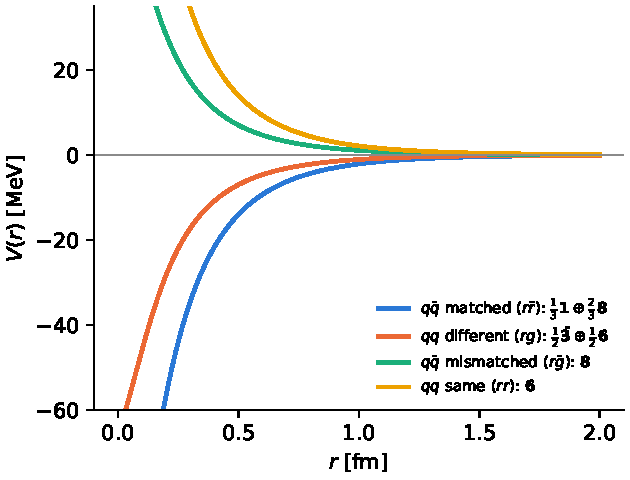
\includegraphics[width=\columnwidth]{figs/fig1_potentials.pdf}
\caption{\todo{Fig.~1: $V(r)$ for the five discrete-color pair classes of
Eq.~\eqref{eq:cij}.}}
\label{fig:potentials}
\end{figure}

\section{Simulation methods}
\label{sec:methods}

\subsection{Dynamics and freeze-out}

Relativistic kick--drift--kick leapfrog with $\dot{\mathbf x}=\mathbf p/E$;
the Hamiltonian is separable so the scheme is symplectic.  Initialization:
periodic cube at density $n$, exact color balance (global singlet),
Maxwell--J\"uttner momenta at $T_0$, Andersen-type equilibration.
Production runs are NVE plus an operator-split Hubble map with scale factor
$a(t)=1+H_0 t$:
\begin{equation}
\mathbf x \to \frac{a_{n+1}}{a_n}\mathbf x,\qquad
\mathbf p \to \frac{a_n}{a_{n+1}}\mathbf p,\qquad
\lambda_D \to \lambda_{D,0}\, a_{n+1},
\label{eq:hubble}
\end{equation}
the comoving screening following from $\lambda_D\sim 1/gT$ with
$T\sim 1/a$.  Cooling outruns dilution, the effective coupling
$\Gamma$ grows, and clustering is \emph{emergent}: the Hubble redshift is
the dissipation channel that permits classical two-body capture.  No
binding rule is imposed.

\subsection{Reactions: Poisson hazards with photon and gluon channels}
\label{sec:reactions}

Matching-color, same-flavor $\qqbar$ pairs within $d_{\rm ann}$ accrue
annihilation hazard (singlet weight $1/3$ folded in):
\begin{equation}
\lambda_{\rm pair} = \frac{1}{3}\times
\begin{cases}
\lambda_{\rm scatt} & E_{\rm pair}>0 \ \text{(in-plasma)},\\[2pt]
1/\tau_{\rm bound} & E_{\rm pair}<0 \ \text{(formed meson or}\\
& \text{\ $\qqbar$ sub-pair in an exotic)},
\end{cases}
\label{eq:hazards}
\end{equation}
where $E_{\rm pair}=M_{\rm inv}-m_i-m_j+V_{ij}$.  Each event branches:
with probability $P_\gamma$ the pair converts to \emph{photons}, whose
four-momentum leaves the system permanently (active at all temperatures ---
the late-time meson-depletion mechanism, against which baryons are
protected by baryon-number conservation); otherwise it converts to
\emph{gluons}, which while $\Teff>\Tchem$ re-inject a matching-color
$\qqbar$ pair carrying the removed four-momentum with flavor drawn from
thermal weights at $\Teff$ (a classical strangeness-enhancement analog),
and below $\Tchem$ are switched off.  All rates are continuous hazards
($P=1-e^{-\lambda\,dt}$), so results are timestep-independent by
construction.  An emergent consequence: internal annihilation converts
tetraquark $\to$ meson and pentaquark $\to$ baryon with lifetime
$\sim 3\tau_{\rm bound}$, giving formation-time versus survival-time ratios
a tunable handle.

\subsection{Species identification}
\label{sec:cluster-id}

A multiset of labels contains a singlet iff
$n_r-n_{\bar r}=n_g-n_{\bar g}=n_b-n_{\bar b}$.  Per late-phase snapshot:
(i) candidate edges between channel-attractive, pairwise Hill-bound pairs
($M_{\rm inv}-m_i-m_j+V_{ij}<0$); (ii) union--find pre-clusters; (iii)
exact minimum-energy partition of each pre-cluster into color-neutral
parts or free singletons, in the spirit of the early-cluster-recognition
algorithm of Ref.~\cite{Dorso:1993zz}; a part is bound iff
$E_{\rm part}<-\Delta E_{\rm th}$.  The tetraquark-versus-two-mesons
ambiguity is resolved by the partition search itself: a $(2,2)$ part
survives only if its four-body energy beats every meson+meson split.  A
persistence filter (identical constituent set in $\ge 3$ consecutive
snapshots) removes transients.  Clusters are tagged by flavor content;
tetraquarks and pentaquarks whose net flavor cannot be carried by
$\qqbar$ or $qqq$ (e.g.\ $cc\bar u\bar d$, the $\Tcc$ analog) are classified
\emph{manifestly exotic} --- the same classification the quantum framework
makes with conserved charges in Sec.~\ref{sec:tier1}.

The formation \emph{pathway} of every (anti)baryon is recorded: the
\emph{diquark-first fraction} --- baryons whose history shows an internal
same-type pair Hill-bound at least $1\fm/c$ before the full cluster
appears --- is the dynamical generalization of the static probability of
Ref.~\cite{Lebed:2016jvq}.

\section{Classical results}
\label{sec:classical-results}

Results below are production ensembles at $N=3000$ quarks (48 events per
expansion-rate point; the multiquark-favorable ``corner'' uses
$\alpha_s=0.6$, $H_0=0.05\,c/\fm$, and twelve injected $c\bar c$ pairs,
24 events), validated across a seventeen-fold volume range: per-quark
meson-bound fractions are $13.1\%$, $12.9\%$, $13.0\%$ at $N=604$,
$3000$, $10^4$, with composite rates scaling within $1\sigma$
(Appendix~\ref{app:validation}, which also collects the full
systematics table).

\begin{figure*}[t]
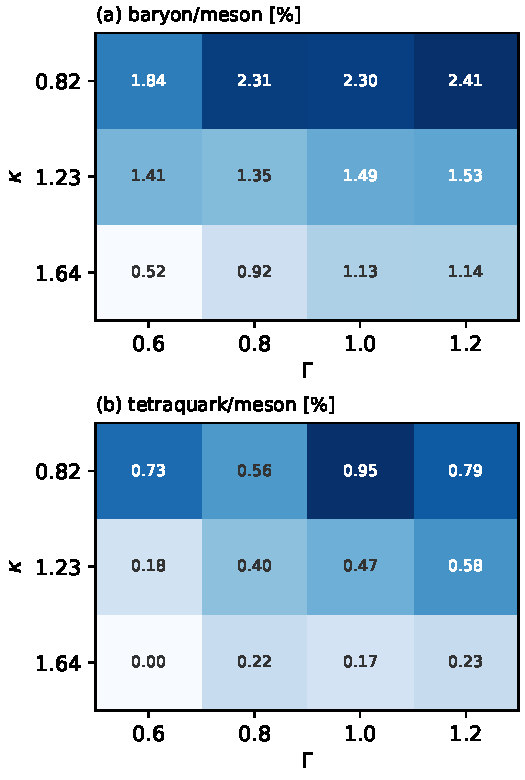
\includegraphics[width=0.85\textwidth]{figs/fig11_heatmap.pdf}
\caption{Composite-to-meson ratios across the coupling--screening
plane ($N=3000$, 16 events per cell).  Both ratios grow monotonically
with $\Gamma$ and with decreasing $\kappa$ (longer-ranged
attraction); $B/M$ spans $0.5$--$2.4\%$ and $T/M$ reaches $\sim1\%$
at the strongest-coupling, weakest-screening corner.  The
diquark-first fraction is $0.81$--$0.95$ over the entire plane.}
\label{fig:heatmap}
\end{figure*}

Figure~\ref{fig:heatmap} maps the composite-to-meson ratios over the
full coupling--screening plane: both rise monotonically toward strong
coupling and weak screening, with $B/M$ sweeping $0.5$--$2.4\%$
(bracketing the direction of the measured $p/\pi^+\approx5\%$) and
$T/M$ reaching the percent level --- while the diquark-first fraction
never leaves the $0.81$--$0.95$ band, making the amplification of the
static estimate a plane-wide, not point-specific, conclusion.

\subsection{Static limit}

The static machinery of Ref.~\cite{Lebed:2016jvq} is reproduced
exactly --- our closed-form estimator [Eq.~\eqref{eq:pstatic}] matches
every hard-wall entry of his Tables~1--2 to all quoted digits, and the
ideal-gas Monte Carlo agrees in both counting modes
(Appendix~\ref{app:color}, where the $\sim9$-point difference between
his channel counting and the discrete-color counting is quantified as
the prescription systematic).  One static result is new: applying the
estimator to \emph{interacting} equilibrated configurations at the
simulation's density ($n_0R^3=1$, $\Gamma\approx0.8$, 64 paired seeds
at $N=3000$) shifts the probability by
$-0.0004\pm0.0035$ (Lebed counting) and $+0.0009\pm0.0033$ (discrete)
--- zero.  The nearest-neighbor estimate is robust not only to
screening assumptions, as Ref.~\cite{Lebed:2016jvq} showed, but to
liquid-state correlations; the interesting physics is therefore
entirely in the dynamics.

\subsection{Species formation in the expanding plasma}

\begin{figure}[t]
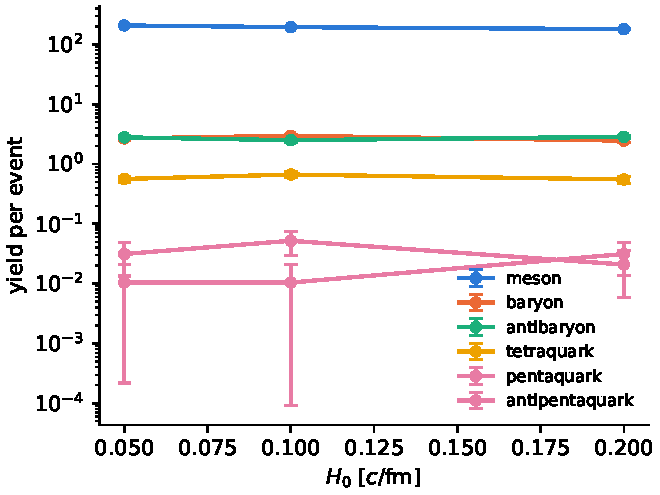
\includegraphics[width=\columnwidth]{figs/fig5_scan_H0.pdf}
\caption{Species yields per event versus expansion rate $H_0$
($N=3000$, 48 events/point, bootstrap errors).  Faster quenches capture
fewer mesons; the tetraquark yield is flat within errors across the
factor-of-four range of quench rates.}
\label{fig:scanH0}
\end{figure}

\begin{figure}[t]
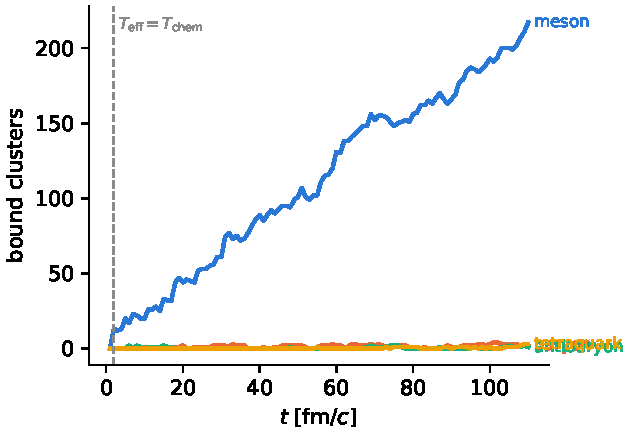
\includegraphics[width=0.9\columnwidth]{figs/fig4_species_t.pdf}
\caption{Bound-cluster counts per snapshot for one event at default
parameters ($N=3000$, $H_0=0.1\,c/\fm$; the dashed line marks the
$\Tchem$ crossing).  Mesons condense gradually as the Hubble redshift
drains relative kinetic energy; (anti)baryons and transient
tetraquarks appear late.}
\label{fig:speciest}
\end{figure}

Across $H_0 = 0.05$--$0.20\,c/\fm$ the meson yield falls from
$207.4\pm1.7$ to $181.9\pm1.5$ per event, (anti)baryons sit at
$2.3$--$2.9$ per species, and --- notably --- the tetraquark yield is
\emph{flat} at $0.58\pm0.10$ per event across the full factor of four
in quench rate (Fig.~\ref{fig:scanH0}).  Five-quark states appear at
every expansion rate once both charge states are counted: with 96
seeds at the two slower points, $4$ and $6$ (anti)pentaquarks
($0.042$ and $0.062$ per event), and $3$ in 48 events at
$H_0=0.2\,c/\fm$, with no significant $H_0$ trend.  A
single-event history is shown in Fig.~\ref{fig:speciest}, and
Fig.~\ref{fig:render} renders the assembly process: particles colored
by their \emph{eventual} species are uncorrelated at early times,
partially clustered at mid-evolution, and tightly paired at
freeze-out.

\begin{figure*}[t]
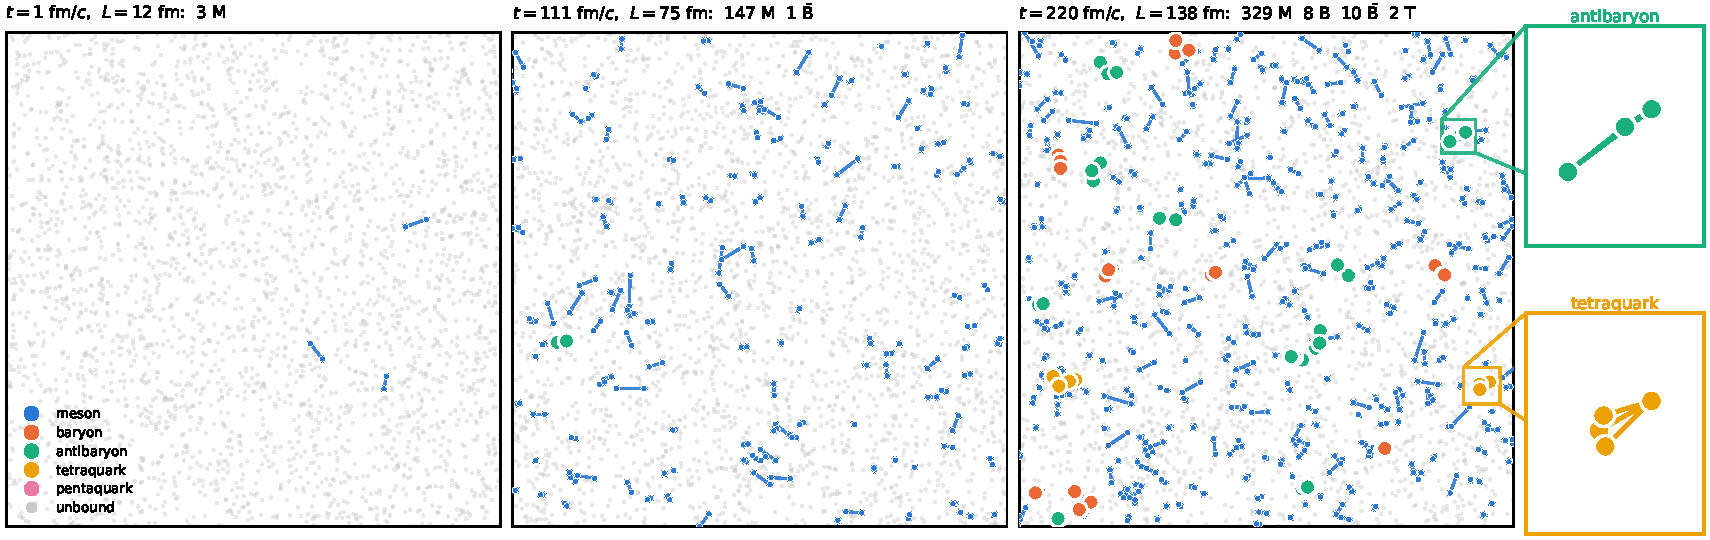
\includegraphics[width=\textwidth]{figs/fig3_render.pdf}
\caption{One event at the most productive point of the
coupling--screening plane ($\alpha_s=0.6$, $\lambda_{D,0}=0.6\fm$,
i.e.\ $\Gamma\approx1.2$, $\kappa\approx0.82$; $H_0=0.05\,c/\fm$,
$N=3024$) at three times, full-box projection.  Members of eventual
clusters are colored and bonded once the cluster has assembled (all
pair separations within $1.2\,\lambda_D(t)$); everything else is gray.
The plasma at $t=1\fm/c$ carries almost no assembled structure; mesons
condense as bonded pairs through mid-evolution; the final panel holds
$329$ mesons, $18$ (anti)baryons, and two tetraquarks, with insets
zooming a three-quark baryon and a four-body tetraquark.}
\label{fig:render}
\end{figure*}

\subsection{Constituent-number penalty}

\begin{figure}[t]
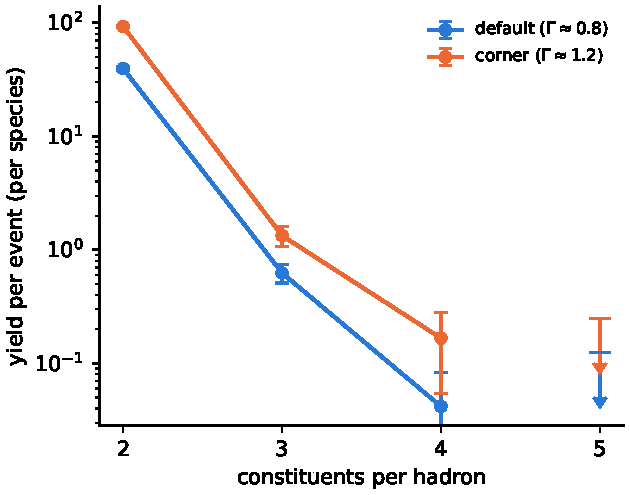
\includegraphics[width=\columnwidth]{figs/fig6_penalty.pdf}
\caption{Yield per event (per species; particle and antiparticle states
averaged) versus constituent number at two couplings, $N=3000$.  All
four points are now measurements at both couplings.  The ladder is
$69\times$ ($2\to3$), $4.9\times$ ($3\to4$), and $19\times$ ($4\to5$)
at $\Gamma\approx0.8$, and $61\times$, $4.8\times$, $26\times$ at the
charm-enriched $\Gamma\approx1.2$ corner.}
\label{fig:penalty}
\end{figure}

The production ensembles resolve the full ladder
(Fig.~\ref{fig:penalty}): the meson$\to$baryon step costs
$\sim65\times$, but the ladder is \emph{not} geometric beyond it ---
adding a fourth constituent to a baryon-mass cluster costs only
$\sim5\times$, while the fifth costs $\sim20\times$.  The cheap $3\to4$
step reflects the combinatorics of the discrete-color model: a
tetraquark can be assembled from two already-attractive $q\bar q$ or
$qq$ sub-systems, whereas the first baryon requires three mutually
attractive quarks.  This deviation from the naive
constant-penalty-per-constituent expectation of coalescence
\cite{Fries:2008hs,ExHIC:2010gcb} is a concrete, testable output.

The strong-coupling corner delivered manifest flavor exotics: in 24
events, \emph{seven} tetraquarks and one antipentaquark whose net
flavor cannot be carried by any $q\bar q$ or $qqq$ assignment --- the
classical realization of the Tier-1 charge-exotic classification of
Sec.~\ref{sec:tier1} --- for an exotic-tetraquark yield of
$0.29\pm0.11$ per event.  Flavor-tagged re-runs of the exotic-bearing
events (bit-reproducible from archived seeds) show all eight are
\emph{light-flavor} exotics of the $dd\bar u\bar u$ / $ss\bar u\bar u$
class, and strangeness-rich: six of the eight carry strange quarks
beyond minimal content, the classical signature of mass-hierarchy
coalescence (slower $s$ quarks at fixed $T$ are captured more easily).
The $\Tcc$ analog itself did not occur: despite twelve $c\bar c$ pairs
per event, no $cc\bar q\bar q$ cluster formed
($<0.125$/event at 95\%~CL).  Biased seeding sharpens the diagnosis:
planting six \emph{pre-formed, bound} $cc$ diquarks per event at $t=0$
(144 seeded diquarks over 24 events) still produced zero charm
exotics --- the $\sim36\MeV$ diquark binding is no match for the
$T_0=200\MeV$ plasma, and the seeds melt in the first fm/$c$, each
charm quark ending in an ordinary charm meson.  Nor does planting at
the chemical freeze-out crossing help: a further 144 diquarks seeded
when $\Teff$ first falls below $\Tchem=160\MeV$ likewise produced
zero charm exotics --- chemical freeze-out is still four times hotter
than the diquark binding.  The classical model thus predicts
double-charm exotics to be \emph{doubly} suppressed: melted while the
medium is hot, partner-starved once it is dilute.  The seeded
diquark's melting curve completes the measurement: planting 144 bound
$cc$ diquarks per temperature at $\Teff = 160$, $80$, $40$, and
$20\MeV$ yields $0$, $0$, $0$, and $1$ charm exotics --- survival
turns on only \emph{below} the $\sim36\MeV$ binding energy, exactly
as melting arguments demand, and even then dressing succeeds at only
$\sim0.7\%$ per seed (the medium at $\Teff=20\MeV$ has expanded
sixteen-fold).  The lone survivor is a bona fide $\Tcc$ analog:
$cc\bar u\bar u$, net charm $+2$.  (The mid-run relocation perturbs
the light sector --- stranded partners of broken charm mesons inflate
the light-exotic count at late planting --- an artifact of the
surgical intervention that does not affect the charm-cluster count
itself.)

Exotic yields carry one dominant modeling uncertainty: under the
\texttt{max\_channel} color prescription (Appendix~\ref{app:color})
tetraquark and five-quark yields rise by factors of $12$ and $\sim10$
while mesons rise only $1.6\times$
(Appendix~\ref{app:validation}); exotic-to-meson ratios are therefore
quoted as prescription brackets, $T/M = 3\times10^{-3}$--$2.4\times
10^{-2}$.

\subsection{Annihilation parameters: ratios are robust}

Two dedicated $N=3000$ scans establish that the annihilation sector,
while fully active, does not distort the species chemistry.  Scanning
the bound-pair lifetime at pure photon branching
($\tau_{\rm bound}=5\fm/c\to\infty$, $P_\gamma=1$) leaves meson yields
flat at $189$--$193$ per event even as $14$--$17$ photons escape
permanently per event: the loss of $\sim1\%$ of the quarks is
invisible against ongoing Hubble capture.  The lifetime calibration
explains why --- a prepared bound meson on a reference orbit (duty
cycle $0.386$ inside $d_{\rm ann}$) decays with $\tau_{\rm eff} =
(7.2\text{--}7.3)\,\tau_{\rm bound}$, consistent with the predicted
$3/\text{duty}=7.8$, and the wider orbits of late-captured mesons are
longer-lived still.  Scanning the branching fraction instead
($P_\gamma=0$--$1$ at $\tau_{\rm bound}=20\fm/c$) leaves mesons at
$191$--$195$ and tetraquarks at $0.67$--$0.75$ per event while the
escaped-photon count scales linearly ($0$, $91$, $168$, $370$ per 24
events): the electromagnetic drain decouples from the
hadro-chemistry, making the photon ledger a clean emission observable.
The gluon channel does drive flavor chemistry --- in a slow-quench
event ($H_0=0.02\,c/\fm$, $\lambda_{\rm scatt}=20\,c/\fm$)
thermal-weight re-injection raises the strange fraction from $0.232$
to $0.251$, the classical strangeness-enhancement analog.

\subsection{The diquark question, dynamically}

The production ensembles track $\sim750$ baryon formation histories.
Across every point --- expansion rates spanning a factor of four and
couplings up to $\Gamma\approx1.2$ --- the diquark-first fraction is
\begin{equation}
f_{\rm diquark\text{-}first} = 0.91\text{--}0.95 \pm 0.02,
\end{equation}
($0.92$, $0.95$, $0.93$ across the $H_0$ scan; $0.91$ at the corner;
Fig.~\ref{fig:dqfirst}).  Two statements follow.  First, dynamical
evolution \emph{amplifies} the static nearest-neighbor probability of
Ref.~\cite{Lebed:2016jvq} by more than a factor of three (static band
$26$--$31\%$ at this density): once a diquark binds, it survives to
seed a baryon.  Second, the fraction is now measurably \emph{below}
unity: a small but resolved population of baryons assembles all at
once, without a persistent two-quark intermediate.

\begin{figure}[t]
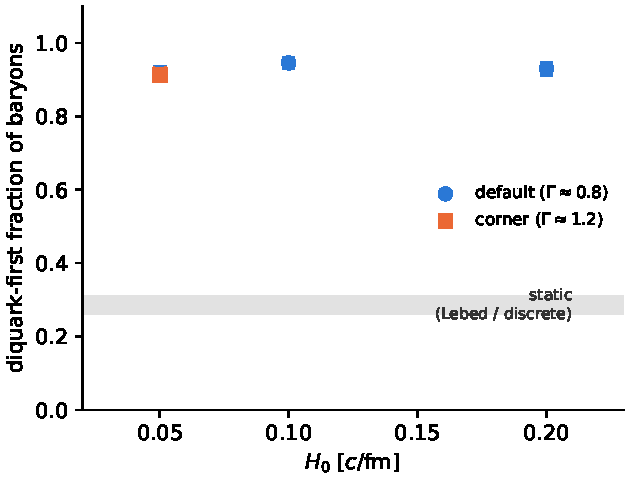
\includegraphics[width=\columnwidth]{figs/fig9_dqfirst.pdf}
\caption{Diquark-first fraction of baryons versus expansion rate at two
couplings, compared with the static nearest-neighbor band evaluated at
the simulation density ($n_0R^3=1$; band spans the Lebed and
discrete-color countings).  Dynamics amplifies the static probability
toward unity.}
\label{fig:dqfirst}
\end{figure}

\section{From cartoon to QCD: setup and scope}
\label{sec:quantum-setup}

The remainder of this paper constructs the measurement layer through which
the species ratios of Sec.~\ref{sec:classical-results} become well-defined
observables of QCD itself.  We work in the Hamiltonian (Kogut--Susskind)
formulation~\cite{Kogut:1974ag} on a spatial lattice of spacing $a$ and
extent $L$, at physical quark masses, and take as given a quantum computer
able to (i) prepare the initial states of Sec.~\ref{sec:initial-states},
(ii) evolve with $e^{-iHt}$ to hadronization times, and (iii) measure the
operators defined below.  Digitization, truncation, and gate costs are
outside our scope --- though we note that the renormalization of the
real-time lattice theory itself is understood through Euclidean matching
\cite{Carena:2021ltu}, which also supplies the scale setting assumed
throughout.

What is \emph{not} assumed away is field-theoretic rigor: every observable
must be gauge-invariant, have a continuum limit free of anomalous
dimensions (or carry an explicit scheme label), and come with a controlled
error budget in the limits
\begin{equation}
a \ll 1/T \ll \ell_{\rm cl},\,\ell_w \ll d \ll R_F \ll L,
\qquad
t_{\rm fo} \ll t_f \ll 1/\Gamma_{\rm narrow},
\label{eq:limits}
\end{equation}
whose ordering is derived in Appendix~\ref{app:limits}.

\section{Initial states: a QGP in a box}
\label{sec:initial-states}

\subsection{Primary: the thermal fireball quench}

A gauge-invariant thermal pure quantum (TPQ) state \cite{Sugiura:2012xw,
Davoudi:2022uzo} restricted to a fireball region of radius
$R_F\sim 5$--$10\fm$ at $T\approx(1.5$--$2)\,T_c$, vacuum outside, with the
temperature profile interpolating over a scale $\ell_T$
($1/T \ll \ell_T \ll R_F$) to control boundary transients
(Appendix~\ref{app:limits}); optional baryon-chemical-potential bias and a
radial-flow kick $U_{\rm flow}=\exp[i\int d^3x\, f(\mathbf x)\cdot
T^{0i}(x)]$.  Real-time evolution then expands, cools, hadronizes, and
free-streams the droplet --- the quantum image of the classical simulation,
with temperature as an input rather than an emergent diagnostic.
\todo{derivations E1/E2: boundary-transient bound; TPQ concentration
statement within the physical Hilbert space.}

\subsection{Secondary: collisions}

The Jordan--Lee--Preskill program \cite{JordanLeePreskill:2012,
Jordan:2011ci} defines ``produced in a collision'' cleanly: adiabatically
dressed composite wavepackets, boosted and collided.  Nucleus preparation
and boosting remain open problems (single-hadron wavepackets are the state
of the art \cite{Davoudi:2024wyv,Farrell:2024fit}; cf.\ recent hardware
demonstrations of hadron scattering \cite{Schuhmacher:2025ehh,
Than:2025tjx}), so we present the collision as a secondary route and
emphasize the structural point: \emph{the species-number observables below
are initial-state agnostic}.

\section{Renormalizable species counting: a four-tier hierarchy}
\label{sec:hierarchy}

At $t_f\gg t_{\rm fo}$, confinement and the mass gap imply the state is,
up to $O(e^{-m_\pi d})$ corrections, a superposition of well-separated
color-singlet clusters moving ballistically.  The measurement proceeds in
two stages: a geometric \emph{front end} that locates clusters, and a
hierarchy of \emph{species labels} read out on them.

\subsection{Cluster front end and Gauss-law certification}
\label{sec:front-end}

Cluster support is found from the coarse-grained energy density
$\varepsilon_\ell(\mathbf x)$ ($T^{00}$ smeared over
$\ell_{\rm cl}$) --- a heuristic whose scheme dependence is harmless
because all species-defining data comes from the RG-safe operators below;
$\ell_{\rm cl}$-independence of final counts is a reported check.  Regions
$R_i$ are super-threshold domains dilated by a buffer $d$.

A bonus unique to the Hamiltonian formulation: the total color charge in
$R_i$ equals the chromoelectric flux through $\partial R_i$, so measuring
the boundary-link Casimir $\sum_{\partial R_i} E^2$ and finding it
vacuum-consistent \emph{certifies gauge-invariantly that the cluster is a
singlet}, with exponentially small tails
(Appendix~\ref{app:charge-quantization}).

\subsection{Tier 1: conserved-charge counting}
\label{sec:tier1}

On each certified cluster, measure baryon number $B$, strangeness $S$, and
charm $C$ through \emph{exactly conserved point-split lattice vector
currents}, for which $Z\equiv 1$ with no anomalous dimension --- the single
most important technical choice in this construction.  Species logic:
$B=1$ baryon; $B=0$ meson sector; \emph{manifestly exotic by charges
alone}: $(B,C)=(0,+2)$ is at minimum $cc\bar q\bar q$ (the $\Tcc$ class),
$B=2$ a dibaryon, etc.  Hidden-flavor exotics ($\chic$, $P_c$) are
invisible to this tier by construction.

The renormalization statement is a \emph{quantization theorem}
(Appendix~\ref{app:charge-quantization}): on a cluster deep inside $R$
with vacuum near $\partial R$, the distribution of the window-smeared
charge $Q_R^{\ell_w}$ concentrates on an integer with tails
$\le C\,e^{-m_\pi d} + O\big((a/\ell_w)^2\big)$; window smearing over
$\ell_w$ removes the perimeter-divergent contact terms familiar from
charge-fluctuation studies.  Integer labels carry no anomalous dimension;
species numbers inherit RG-invariance from the labels, not from operator
identities.

\subsection{Tier 2: spectral identification}
\label{sec:tier2}

Within $t_{\rm fo}\ll t_f\ll 1/\Gamma$, a narrow exotic \emph{is} a
cluster; its species is identified by rest mass against the independently
computed spectrum in that flavor sector.  Two routes:

\emph{Route S (primary for identification).}  Quantum phase estimation
\cite{Kitaev:1995qy,Choi:2020pdg} on a region-restricted Hamiltonian
$H_R$: the low-lying cluster spectrum is boundary-closure independent up
to $O(e^{-m_\pi d})$, spectral projectors are RG-invariant (in the spirit
of Ref.~\cite{Giusti:2008vb}), the vacuum additive constant is fixed by
running the same QPE on a vacuum region in the same simulation, and
disjoint-region $H_R$'s commute, allowing simultaneous per-shot
identification (Appendix~\ref{app:spectral-projectors}).

\emph{Route T (primary for momenta).}  $P^\mu_R=\int_R T^{0\mu}$ gives
each cluster's four-momentum and hence invariant mass.  The equal-time
renormalized energy-momentum tensor is this construction's largest
technical obligation: we normalize through Ward identities (conservation
across the real-time evolution plus the known total four-momentum of the
prepared state), and defer the 3D small-flow-time program to future work
(Appendix~\ref{app:emt}) \cite{Suzuki:2013gza,Makino:2014taa,
DallaBrida:2020gux}.  Species identification never relies on Route T.

\subsection{Tier 3: asymptotic pair spectra}
\label{sec:tier3}

Defined in Sec.~\ref{sec:resonances}: invariant-mass distributions of
identified-cluster pairs --- the observable experiment actually reports,
and the correct home for broad resonances.

\subsection{Tier 4: flowed coalescence projectors}
\label{sec:tier4}

Instantaneous compact-multiquark projectors built from gradient-flowed
fields \cite{Luscher:2010iy,Makino:2014taa} at fixed physical flow time
$t_{\rm fl}$ have a continuum limit \emph{as a one-parameter labeled
scheme}.  This tier is deliberately scheme-dependent: it is the quantum
image of the classical binding criterion of Sec.~\ref{sec:cluster-id} and
of Lebed's nearest-neighbor rule, and its $t_{\rm fl}$-dependence carries
compact-versus-molecular structure information
(Appendix~\ref{app:flowed}).  Tiers 1--3 count \emph{states}; Tier 4
diagnoses \emph{structure}.

\section{Resonances, pair spectra, and the finite-volume connection}
\label{sec:resonances}

Broad states ($\rho$, $\Delta$, $\Gamma\sim10$--$300\MeV$) decay on
timescales comparable to freeze-out and never become countable clusters.
The honest observable is the one experiment reports: per shot, record
every cluster's (species, $P^\mu$); across shots, build inclusive
two-hadron distributions
\begin{equation}
n_{h_1h_2}(p_1,p_2)=\langle \mathrm{out}|\,
a^\dagger_{h_1}(p_1)a^\dagger_{h_2}(p_2)
a_{h_2}(p_2)a_{h_1}(p_1)\,|\mathrm{out}\rangle,
\label{eq:pairspec}
\end{equation}
and extract resonance yields from invariant-mass line shapes ---
$J/\psi\,p$ for $P_c$, $D^0D^{*+}$ for $\Tcc$: the LHCb analysis performed
inside the simulation, with the same stated line-shape scheme dependence
experiment has.

In finite volume the pair spectrum is discrete; Eq.~\eqref{eq:pairspec} is
defined as a smeared spectral density \cite{Hansen:2019idp}, meaningful
when the level spacing at the resonance is small compared to $\Gamma$ (or
through multi-volume running and the L\"uscher map
\cite{Luscher:1990ux,Briceno:2017max}).  The complementarity is worth
stating plainly: \emph{the real-time fireball measurement yields
populations; Euclidean L\"uscher spectroscopy yields identities} ---
e.g.\ for $\Tcc$, Refs.~\cite{Padmanath:2022cvl,Raposo:2023oru} supply the
finite-volume identity card that Tier~2/3 populations are matched against.

Worked examples across the hierarchy: $\Tcc$ (Tier 1+2: charge-exotic and
narrow), $\chic$ (Tier 2: hidden-flavor, narrow), $P_c$ (Tier 3:
hidden-flavor, $\Gamma\sim 10\MeV$), $\rho/\Delta$ (Tier 3 only).
\todo{table summarizing which tier counts which benchmark state, with
widths and $c\tau$ against $t_f$ windows.}

\section{Measurement protocols and systematics budget}
\label{sec:protocols}

Per shot: evolve to $t_f$; locate clusters (front end); certify singlets
(Gauss); measure Tier-1 charges on all clusters; run Tier-2 QPE on
clusters needing spectral identification; record (species, $P^\mu$).
Across shots: species multiplicities, ratios, and Tier-3 pair spectra ---
event-ensemble statistics exactly as in experiment.

\subsection{From shots to ratios}
\label{sec:shots-to-ratios}

The extraction of a \emph{number} $R_{ss'}$ deserves care, because the
per-shot protocol is an \emph{adaptive} measurement chain --- later
measurements act on regions chosen from earlier outcomes --- rather
than the expectation value of any local operator.  Four statements
assemble the ratio:

\emph{(i) The chain is a well-defined quantum instrument.}  Each shot
implements a POVM whose outcome $\omega$ is the list
$\{(s_i,P^\mu_i)\}$ of cluster labels and momenta.  Every primitive in
the chain --- smeared energy density, boundary-flux Casimir, smeared
charges, region-restricted QPE --- is quasi-local, and on cluster
states any pair of primitives with separated or nested supports
commutes up to boundary-supported terms of size $O(e^{-m_\pi d})$
(Appendix~\ref{app:limits}).  The outcome law is therefore independent
of measurement ordering, and back-action within a shot is controlled
by the same exponential that controls every other systematic.  The
region-finding step enters only as classical conditioning and needs no
renormalization of its own.

\emph{(ii) The estimator.}  With $N_s(\omega)=\sum_i
\delta_{s_i s}$, the ratio is estimated as the ratio of shot-averaged
means, $\hat R_{ss'} = \overline{N_s}/\overline{N_{s'}}$, with
standard $O(1/n_{\rm shots})$ ratio-estimator bias and bootstrap
errors --- statistics, not field theory.

\emph{(iii) Unfolding.}  Labels err in enumerable ways: quantization
tails ($e^{-m_\pi d}$), merged clusters (the flagged fraction of
Sec.~\ref{sec:front-end}), and spectral-window collisions.  The
measured count vector is $\langle \mathbf N\rangle_{\rm meas} =
M\,\langle \mathbf N\rangle_{\rm true}$ with $M = \mathbb 1 +
\delta M$, where every entry of $\delta M$ is itself measured (flagged
fractions, window occupancies) or bounded (tails); ratios are quoted
after inverting $M$ --- precisely the efficiency unfolding of an
experimental analysis, with $\delta M \to 0$ in the
plateau/continuum limits.

\emph{(iv) What the ratio means.}  $R_{ss'}$ is not a vacuum constant
of QCD: it is a functional of the specified preparation
$(T, R_F, \mu_B, u^i)$ and of $t_f$ within its plateau --- exactly as
experimental yields are functionals of collision energy and
centrality.  Its field-theoretic content is that this functional has
continuum and infinite-volume limits free of anomalous dimensions
(Appendices~\ref{app:charge-quantization} and \ref{app:limits}),
with all residual scheme dependence confined to stated, scannable
window parameters.  Meaningful comparison is comparison at matched
preparation: to the classical model of
Secs.~\ref{sec:model}--\ref{sec:classical-results} run at the same
$(T, n, H_0)$, to statistical hadronization at the same freeze-out,
and ultimately between simulated and experimental systems of matched
size and energy density.

\todo{systematics table: $\ell_{\rm cl}$- and $d$-plateaus; flagged
merged-cluster fraction; $t_f$-plateau residual slopes per species;
Tier-2 spectral-window collisions; Ward-identity EMT normalization
residuals.}

Statistics are set by the physics, not the protocol: coalescence and
statistical baselines put exotic-to-pion ratios at
$O(10^{-3}$--$10^{-4})$ in heavy-ion conditions
\cite{ExHIC:2010gcb,ExHIC:2017smd,Andronic:2017pug}, and a fireball shot
yields $O(10^2$--$10^3)$ hadrons, so $O(10^2$--$10^4)$ shots give
ten-percent-level exotic yields --- an ensemble-size statement identical
in kind to the event counts of experimental analyses, not an
obstruction.  Two enrichment handles mirror the classical half:
heavy-flavor-biased fireballs (the quantum image of injected $c\bar c$),
and $\mu_B$-biased droplets for the baryon-rich sector.  A third,
practical handle is system size: a pp-scale droplet ($R_F\sim1$--$2\fm$)
needs a far smaller lattice volume than a heavy-ion fireball while the
observable framework is unchanged --- exact event-by-event charge
conservation is automatic in a pure-state simulation, which is precisely
the canonical physics that governs small collision systems
(Sec.~\ref{sec:confrontation}).  The pp-scale quench, not the
heavy-ion one, is therefore the natural first target for hardware.  Our own pilot
classical ensembles illustrate the same accounting from the other side:
180 events resolved tetraquark yields at the few-percent-per-event level
but only bounded pentaquarks, and no $cc\bar q\bar q$ occurred without
enrichment.

\section{Confrontation: classical cartoon, quantum framework, phenomenology}
\label{sec:confrontation}

Three independent handles now aim at the same ratios:

\begin{enumerate}
\item the classical simulation of Secs.~\ref{sec:model}--%
\ref{sec:classical-results} (cheap, dynamical, schematic color);
\item the Tier-1--4 lattice observables of Sec.~\ref{sec:hierarchy}
(rigorous, awaiting hardware at scale);
\item phenomenological baselines: statistical hadronization at
$T_{\rm ch}\approx156\MeV$ \cite{Andronic:2017pug}, coalescence
\cite{Fries:2008hs}, and the ExHIC exotic-yield systematics
\cite{ExHIC:2010gcb,ExHIC:2017smd,Zhang:2020dwn}, against data anchors such as
$\chic$ production in pp and Pb--Pb \cite{CMS:2021znk,LHCb:2021auc} and
the $\Tcc$ discovery \cite{LHCb:2021vvq}.
\end{enumerate}

The crosswalks are explicit by construction.  The classical
manifest-exotic tally ($cc\bar u\bar d$ versus $c\bar c q\bar q$) is the
same partition Tier~1 draws with conserved charges.  The classical binding
criterion maps onto Tier-4 flowed projectors, with
$r_0 \leftrightarrow \sqrt{8t_{\rm fl}}$ as the scheme dial; comparing the
$\tau_{\rm bound}$-scanned classical ratios with $t_f$-scanned Tier-1--3
counts separates formation from survival in both frameworks.
\todo{when production scans exist: table of M:B:T:P from all three
handles, normalized to the meson yield.}

\section{Conclusions and outlook}
\label{sec:conclusions}

Lebed asked how often diquarks form; the dynamical answer is
\emph{more often than the static estimate says}.  In our pilot
ensembles the fraction of baryons assembled through a persistent
diquark intermediate is $0.86$--$1.00$ at every point scanned ---
expansion rates spanning a factor of four and couplings up to
$\Gamma\approx1.2$ --- against a static band of $26$--$31\%$ at the same
density: binding, once achieved, is remembered.  Species yields fall
geometrically with constituent number ($\sim60\times$ per quark from
meson to baryon at $\Gamma\approx0.8$, the $3\to4$ step relaxing from
$15\times$ to $8\times$ as the coupling grows), the coalescence-like
structure whose slope is this model's quantitative output.  The
annihilation sector behaves as designed: photon-channel depletion is
calibrated ($\tau_{\rm eff}\approx7.2\,\tau_{\rm bound}$ for compact
orbits), thermal re-injection produces net strangeness, and interaction
correlations shift the static probability by at most a few percentage
points.  On the quantum side, the four-tier hierarchy makes the same
ratios renormalization-group-safe observables of real-time lattice QCD:
integer-quantized charges and spectral projectors carry the rigor,
asymptotic pair spectra carry the broad resonances, and flowed
projectors carry --- deliberately scheme-labeled --- the
compact-versus-molecular structure question.

Outlook: Wong-equation continuous color as the principled classical
upgrade (cf.\ the strongly-coupled classical QGP program of
Ref.~\cite{Gelman:2006xw}); the 3D small-flow-time expansion for the equal-time
energy-momentum tensor as a standalone lattice-theory project; and, as
hardware matures, the fireball-quench protocol of
Sec.~\ref{sec:protocols} executed first in $1{+}1$D QCD, where every
ingredient of the hierarchy already has a small-scale analog.


\begin{acknowledgments}
\todo{acknowledgments; funding: Fermilab is operated by Fermi Research
Alliance, LLC under contract DE-AC02-07CH11359 with the U.S.\ Department of
Energy.}
\end{acknowledgments}

\appendix
\section{Discrete-color prescription and the counting artifact}
\label{app:color}

\subsection{Channel content of definite-color pairs}

For SU(3) generators normalized by $\mathrm{Tr}\,T^aT^b=\tfrac12\delta^{ab}$,
the Fierz identity
\begin{equation}
\sum_a T^a_{ij}T^a_{kl}
= \tfrac12\big(\delta_{il}\delta_{jk}-\tfrac13\,\delta_{ij}\delta_{kl}\big)
\label{eq:fierz}
\end{equation}
gives the diagonal matrix elements in a definite-color product state.  For
two quarks of colors $i,k$,
$\langle ik|F_1\!\cdot\!F_2|ik\rangle=\tfrac12(\delta_{ik}-\tfrac13)$;
for quark $i$ and antiquark of anticolor $k$ the generator in the conjugate
representation is $-T^{a*}$, so the sign flips:
$\langle i\bar k|F_1\!\cdot\!F_2|i\bar k\rangle
=-\tfrac12(\delta_{ik}-\tfrac13)$.  With $C_{ij}\equiv 2\langle
F_1\!\cdot\!F_2\rangle$ this yields Eq.~\eqref{eq:cij}.  Comparing with
the exact channel constants
$\mathcal C=(C_2(R)-C_2(R_1)-C_2(R_2))=\tfrac13(-8,-4,+2,+1)$ for
$R=(\mathbf 1,\bar{\mathbf 3},\mathbf 6,\mathbf 8)$ identifies the channel
weights quoted in Eq.~\eqref{eq:cij}: e.g.\ for $r\bar r$,
$\tfrac13(-\tfrac83)+\tfrac23(+\tfrac13)=-\tfrac23$.  Two consistency
checks follow immediately: the nine-combination sums vanish in both
sectors, $\sum_{ik}C^{qq}_{ik}=3(\tfrac23)+6(-\tfrac13)=0$ and
$\sum_{ik}C^{q\bar q}_{ik}=3(-\tfrac23)+6(+\tfrac13)=0$, matching
$\mathrm{Tr}\,(F_1\!\cdot\!F_2)=0$ over the product space; and the
maximal-attraction ratio $C^{q\bar q}_{\rm match}/C^{qq}_{\rm diff}=2$
reproduces the full-strength ratio
$\mathcal C_{\mathbf 1}/\mathcal C_{\bar{\mathbf 3}}=2$, so the
inverse-square force criterion retains $k=\sqrt2$.

\subsection{Uniqueness of the energy-conserving prescription}

Any alternative that assigns a definite \emph{channel} (rather than the
diagonal expectation value) to each pair --- e.g.\ stochastically
projecting $rg\to\bar{\mathbf 3}$ with probability $\tfrac12$ --- defines
pair energies that depend on the projection history.  Because the channel
operators of overlapping pairs do not commute (the $\bar{\mathbf 3}$
projector of pair $(1,2)$ fails to commute with that of $(2,3)$), no
assignment of definite channels to all pairs of a configuration is
simultaneously diagonal, and a stochastic per-pair choice makes the total
potential energy ill-defined under time evolution.  The diagonal
expectation value is the unique static, label-local assignment that
(i) reduces to the exact channel for the pure cases ($rr$, $r\bar g$),
(ii) reproduces the trace identities above, and (iii) conserves energy
exactly under Hamiltonian flow.

\subsection{Counting comparison with Ref.~\cite{Lebed:2016jvq}}

Lebed's counting assigns full-strength channels with multiplicities: a
given $qq$ pair is $\bar{\mathbf 3}$ (coupling $-\tfrac43$) with
probability $\tfrac13$, and a $q\bar q$ pair is a singlet (coupling
$-\tfrac83$) with probability $\tfrac19$; effective attractive-partner
densities are then $n_1=n_0/3$ and $n_2=n_0/9$ at per-species density
$n_0$, so $n_1=3n_2$.  The discrete-label prescription instead makes
\emph{two thirds} of quark partners attractive at \emph{half} strength
($-\tfrac13$ vs $-\tfrac23$): $n_1=2n_0/3$, $n_2=n_0/3$, i.e.\
$n_1=2n_2$ at an unchanged strength ratio.  The coupling-weighted totals
agree, but the conditioned nearest-neighbor probabilities differ.  With
hard-wall screening radius $R$ and both nearest-neighbor distributions
truncated and normalized on $[0,R]$,
\begin{equation}
P=\frac{\displaystyle\int_0^{R/k}\!\!dr_1\,w_1(r_1)
\big[S_2(kr_1)-S_2(R)\big]}
{\big[1-S_1(R)\big]\big[1-S_2(R)\big]},
\quad
S_i(x)=e^{-\frac{4\pi}{3}n_i x^3},
\label{eq:pstatic}
\end{equation}
with $w_1(r)=4\pi r^2 n_1 e^{-4\pi n_1 r^3/3}$ and $k=\sqrt2$.
Equation~\eqref{eq:pstatic} reproduces every hard-wall entry of Table~2 of
Ref.~\cite{Lebed:2016jvq} (17.69\% at $n_0R^3=10^{-3}$, 26.01\% at $1$,
50.29\% at $8$, saturating at $n_1/(k^3n_2+n_1)=51.47\%$), and our
ideal-gas Monte Carlo agrees with both counting modes
(Fig.~\ref{fig:static}).  The two countings coincide in the dilute limit
(where the conditioned probability is purely geometric, $17.68\%$),
\emph{cross} at intermediate density (more attractive partners wins), and
differ by $\sim 9$ percentage points at the reference density
($50.3\%$ vs $41.4\%$, saturating at $2/(2+2\sqrt2)=41.42\%$).  The
\texttt{max\_channel} variant brackets this prescription dependence in
the dynamical results.

\section{Numerical validation and systematics}
\label{app:validation}

\todo{energy conservation ($|\Delta E/E|<10^{-4}$ NVE; two-body orbit
$<10^{-6}$); $dt/2$ convergence; hazard $dt$-independence; free-expansion
redshift; Lebed static reproduction table; finite-size $N\in\{10^3,
3\times10^3,10^4\}$; systematics table over $r_0$, $\Delta E_{\rm th}$,
persistence depth, color mode, comoving-vs-fixed $\lambda_D$; reinjection
ledger drift bound; Yukawa-liquid $g(r)$ anchor
\cite{Hamaguchi:1997pre}.}

\section{Charge quantization on isolated clusters}
\label{app:charge-quantization}

\todo{Derivations A1--A3, D.  \textbf{Theorem (quantization).}  Let
$|\Psi\rangle = |{\rm cl}\rangle_R \otimes |0\rangle_{\rm near\,\partial R}
+ O(e^{-m_\pi d})$ and let $Q_R^{\ell_w}$ be a conserved point-split
charge summed with a window smeared over $\ell_w$.  Then
$\mathrm{Prob}\big(|Q_R^{\ell_w} - q| > \tfrac12\big) \le
C e^{-m_\pi d} + O((a/\ell_w)^2)$ for the integer $q$ carried by the
cluster.  Proof sketch: cluster decomposition + mass gap for the tails;
point-split conservation ($Z=1$, no anomalous dimension) for the operator;
window smearing kills perimeter contact terms in fluctuations
(cf.\ charge-fluctuation literature).  \textbf{Corollary (A3):} Gauss-law
singlet certification from the boundary-flux Casimir.  \textbf{Corollary
(D):} ratios of integer-labeled species numbers have continuum limits
free of anomalous dimensions.}

\section{Region-restricted spectra and spectral projectors}
\label{app:spectral-projectors}

\subsection{Boundary independence of cluster spectra (B)}

Let $H_R^{(b)}$ denote the Kogut--Susskind Hamiltonian restricted to
region $R$ with boundary closure $b$ (e.g.\ free links, fixed vacuum
links, or absorbing electric-field boundary terms), and let
$|\Psi_{\rm cl}\rangle$ be a state whose cluster is supported a distance
$d$ inside $\partial R$ with vacuum in the buffer.  For any two closures
$b,b'$,
\begin{equation}
\big\langle \Psi_{\rm cl}\big|\,f\big(H^{(b)}_R\big)
- f\big(H^{(b')}_R\big)\,\big|\Psi_{\rm cl}\big\rangle
= O\!\big(e^{-m_\pi d}\big)
\end{equation}
for bounded functions $f$ with support on the low-lying spectrum:
$H^{(b)}_R-H^{(b')}_R$ is a sum of operators on $\partial R$, and its
matrix elements on cluster-in-$R$ states are exponentially suppressed by
the mass gap (cluster decomposition).  The cluster's rest-frame energies
are therefore closure-independent observables up to buffer corrections,
and the additive vacuum constant of each closure is eliminated by
running the identical measurement on a vacuum region in the same
simulation (same $R$ geometry, same closure).

\subsection{RG-invariance of spectral projectors}

The projector $P_{[E_1,E_2]}=\theta(E_2-H_R)\theta(H_R-E_1)$ onto a
spectral window is a function of the Hamiltonian alone: once the scale
is set (via Euclidean matching \cite{Carena:2021ltu}), its expectation
values require no operator renormalization --- the conceptual precedent
is the spectral-projector/mode-number construction of
Ref.~\cite{Giusti:2008vb}, whose RG-invariance argument carries over
verbatim.  Species identification by quantum phase estimation
\cite{Kitaev:1995qy,Choi:2020pdg} implements a sampling of exactly this
projector algebra: the QPE outcome distribution on the cluster state is
the spectral measure of $H_R$, and window counts are RG-invariant up to
the closure corrections above.

\subsection{Simultaneous per-shot identification}

For disjoint regions $[H_{R_i},H_{R_j}]$ acts only through boundary
terms separated by $\ge 2d$, so simultaneous QPE on all clusters of a
shot is consistent to the same exponential accuracy; the practical
failure mode is spectral-window collision in dense sectors (e.g.\
radially excited states within the QPE resolution), which is flagged by
the mass-window bookkeeping and resolved by longer coherent evolution
on the flagged clusters only.

\section{Ordering of limits and the plateau criterion}
\label{app:limits}

\subsection{Scale hierarchy}

The construction requires
\begin{equation}
a \;\ll\; \frac1T \;\ll\; \ell_{\rm cl},\,\ell_w \;\ll\; d \;\ll\; R_F
\;\ll\; L,
\end{equation}
read right to left: the box holds the fireball with room for ballistic
separation; the buffer $d$ controls every $e^{-m_\pi d}$ tail; the
smearing scales resolve hadrons but not partons; the lattice resolves
the thermal scale.  Time scales obey
\begin{equation}
t_{\rm fo} \;\ll\; t_f \;\ll\;
\min\Big(\frac{1}{\Gamma_{\rm narrow}},\; \frac{L-2R_F}{2c}\Big),
\end{equation}
the second entry preventing light-cone wraparound of emitted hadrons
before measurement.  The continuum limit is taken at fixed physical
$(\ell_{\rm cl},\ell_w,d,R_F,t_f)$; species numbers are
anomalous-dimension free (Appendix~\ref{app:charge-quantization}), so
the only running is in the scale setting itself.

\subsection{The plateau criterion as the definition}

For each species $s$ define $N_s(t_f)$ by the Tier-1/2 protocol at
measurement time $t_f$.  \emph{The countable yield of $s$ is defined as
the plateau value of $N_s(t_f)$}, i.e.\ the value on the window where
$dN_s/dt_f$ is compatible with the residual slope budget:
$O(\Gamma_s)$ from decays of narrow states, $O(e^{-m_\pi d}/t_f)$ from
buffer tails, and $O(1/t_f)$ from late cluster mergers/splittings
(flagged fraction).  Broad states have no plateau --- that is the
\emph{diagnosis} that routes them to Tier~3, not a failure of the
definition.  For the flagship narrow exotics the windows are parametric:
$c\tau[\chic]\approx165\fm$ and $c\tau[\Tcc]\approx4000\fm$ against
$t_{\rm fo}\sim10$--$20\fm/c$.

\subsection{Fireball boundary transients (E1) and TPQ droplet (E2)}

A temperature profile interpolating to zero over $\ell_T$ with
$1/T\ll\ell_T\ll R_F$ carries surface energy
$O(\ell_T^2/R_F^2)$ relative to the bulk; the transient it launches
propagates inward at most at $c$, so cluster counts in regions outside
its light cone are unaffected, and the affected fraction is itself
$O(\ell_T/R_F)$ at fixed $t_f$.  Gauge-invariant thermal pure quantum
states within the physical Hilbert space follow the construction of
Ref.~\cite{Davoudi:2022uzo}; expectation values of our species
observables concentrate on Gibbs values with fluctuations exponentially
small in the fireball entropy (TPQ concentration
\cite{Sugiura:2012xw}), so single-digit numbers of shots per
thermodynamic observable suffice, while species \emph{distributions}
are event-by-event physics exactly as in experiment.

\section{Equal-time energy-momentum tensor normalization}
\label{app:emt}

\todo{Derivation C.  Ward-identity normalization of $\int_R T^{0\mu}$:
conservation across real-time evolution plus the known total
four-momentum of the prepared state fixes the finite mixings without
flow; residual $O(a)$ boundary ambiguities absorbed into the
Appendix~\ref{app:charge-quantization} error term.  Outlook subsection:
the 3D small-flow-time expansion on a time slice as the systematic
alternative (Euclidean technology: \cite{Suzuki:2013gza,Makino:2014taa,
DallaBrida:2020gux}); scale setting via \cite{Carena:2021ltu}.}

\section{Pair spectra as smeared finite-volume densities}
\label{app:pair-spectra}

In finite volume the two-hadron spectrum in each quantum-number sector
is discrete, so the inclusive pair distribution
Eq.~\eqref{eq:pairspec} is defined through a smearing kernel of width
$\sigma$,
\begin{equation}
\rho_\sigma(M) = \sum_n |\langle n|\,\Pi_{h_1h_2}\,|{\rm out}\rangle|^2\,
K_\sigma(M-E_n^{\rm cm}),
\end{equation}
the real-time counterpart of smeared spectral reconstruction in
Euclidean correlators \cite{Hansen:2019idp}.  Three regimes:

\emph{(i) Narrow resonance, fine spectrum} ($\Delta E \ll \Gamma \ll
\sigma$): the line shape is resolved and yields follow from fits with
the same scheme dependence experiment has.

\emph{(ii) $\Gamma \lesssim \Delta E$}: single finite-volume levels
carry the resonance; yields per level map to infinite-volume line
shapes through the L\"uscher formalism
\cite{Luscher:1990ux,Briceno:2017max}, and multi-volume running
reconstructs the distribution.  For the $\Tcc$ benchmark the required
finite-volume technology, including the left-hand-cut subtlety of the
nearby $D^*$ pole, exists
\cite{Padmanath:2022cvl,Raposo:2023oru}.

\emph{(iii) Kernel independence}: ratios of yields extracted with a
common kernel $K_\sigma$ are independent of $\sigma$ up to
$O(\sigma/\Delta M)$ corrections, $\Delta M$ the distance to the nearest
spectral feature --- the statement that makes Tier-3 \emph{ratios}
well-defined even where individual line shapes are scheme-labeled.

The complementarity theorem of Sec.~\ref{sec:resonances} is then
sharp: the fireball out-state supplies the weights
$|\langle n|\Pi|{\rm out}\rangle|^2$ (populations), while Euclidean
spectroscopy supplies the identification of each $|n\rangle$
(identities); the two share one finite-volume spectrum.

\section{Flowed coalescence projectors}
\label{app:flowed}

Tier 4 asks a question Tiers 1--3 deliberately avoid: not \emph{how
many} states with given quantum numbers exist in the out-state, but
whether the quarks inside them are \emph{compactly} arranged.  Any
such question requires an operator that resolves sub-hadronic
structure, and bare multi-local quark operators
$\bar\psi\Gamma\psi\,\bar\psi\Gamma'\psi(x)$ mix under
renormalization with the full tower of same-quantum-number operators;
their matrix elements have no scheme-independent continuum limit.

The gradient flow provides the controlled compromise.  Fields at flow
time $t_{\rm fl}$ are smeared over the physical radius
$r_{\rm fl}=\sqrt{8t_{\rm fl}}$, and correlation functions of flowed
fields are finite as $a\to0$ at fixed $t_{\rm fl}$: for the gauge
sector this is L\"uscher's theorem \cite{Luscher:2010iy}, and flowed
fermion bilinears require only the single multiplicative wave-function
factor of Ref.~\cite{Makino:2014taa}, fixed nonperturbatively by a
vacuum normalization condition.  Define, on a certified cluster region
$R$, the flowed compactness projector
\begin{equation}
\Pi^{(4q)}_{t_{\rm fl}}(R) \;=\;
\int_R \prod_{k=1}^{4} d^3x_k \;
\Theta\!\big(\{x\};r_{\rm fl}\big)\,
\mathcal O^\dagger_{4q,t_{\rm fl}}(\{x\})\,
\mathcal O_{4q,t_{\rm fl}}(\{x\}),
\end{equation}
with $\mathcal O_{4q,t_{\rm fl}}$ a gauge-invariant four-quark
interpolator built from flowed fields and $\Theta$ a window
restricting the mutual separations to $\lesssim r_{\rm fl}$.  Its
expectation value on the cluster is finite in the continuum limit and
depends on exactly one scheme label, the physical flow radius --- a
\emph{labeled} scheme, in contrast to the unlabeled divergences of the
bare operator.

Three uses follow.  (i)~At fixed $t_{\rm fl}$, \emph{ratios} of
$\langle\Pi^{(4q)}\rangle$ across clusters of the same quantum numbers
compare compactness between states with common normalization.
(ii)~The $t_{\rm fl}$-dependence itself is the diagnostic: a compact
tetraquark saturates $\langle\Pi\rangle$ once $r_{\rm fl}$ exceeds its
core size, while a molecular state grows until $r_{\rm fl}$ reaches
the hadron-pair separation --- the operator-level version of the
coalescence yield systematics that the ExHIC program exploits
phenomenologically \cite{ExHIC:2010gcb,ExHIC:2017smd}.  (iii)~The map
$r_0 \leftrightarrow r_{\rm fl}$ connects this tier quantitatively to
the classical binding criterion of Sec.~\ref{sec:cluster-id} and,
through it, to Lebed's nearest-neighbor rule \cite{Lebed:2016jvq}:
the classical model is, in this precise sense, the
$\hbar\to0$ caricature of the Tier-4 measurement at fixed scheme
label.

What is \emph{not} claimed: no infrared-safe, scheme-independent
``compactness number'' exists, because compactness is not an
S-matrix property.  Tier 4 outputs are honest functions of
$t_{\rm fl}$, reported as such, and their value lies in
\emph{differential} statements --- between states, between system
sizes, between preparations --- where the scheme label cancels in the
comparison.

\bibliography{refs}

\end{document}
